\documentclass{article}
\usepackage{tikz}
\usepackage{csquotes}
\usepackage{mhchem}
\usepackage[a4paper]{geometry}
\usepackage{fancyhdr}
\pagestyle{fancy}
\lhead{Synapsen}
\rhead{Dezember 2025}
\begin{document}
\section{Synapsen}
Das Ende einer jeden Nervenzelle, genannt die \emph{präsynaptische Endigung} oder \emph{Endknöpfchen}, sind verdickt. Darauf folgt der \emph{synaptische Spalt}, danach die Folgezelle. Dies bildet eine Synapse. 
\begin{center}
\tikzset{samples=10} 
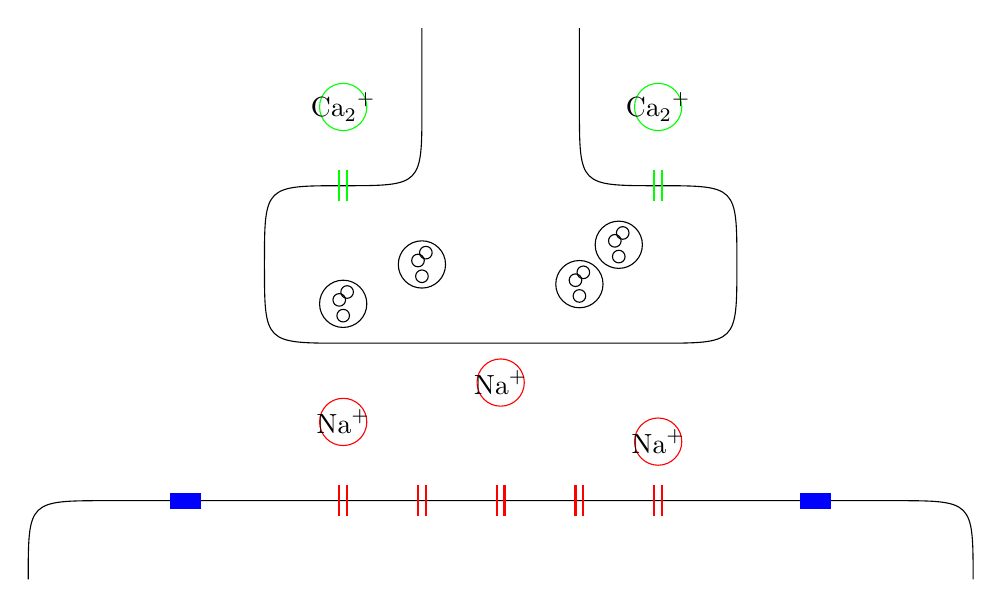
\begin{tikzpicture}
 \newcommand{\channel}[3]{
  \draw[#3, thick] (#1-0.05, #2-0.2) -- (#1-0.05, #2+0.2);
  \draw[#3, thick] (#1+0.05, #2-0.2) -- (#1+0.05, #2+0.2);
 }
 
 \newcommand{\vesikel}[2]{
  \draw (#1, #2) circle (0.3cm);
  \draw (#1, #2-0.15) circle (0.08cm);
  \draw (#1+0.05, #2+0.15) circle (0.08cm);
  \draw (#1-0.05, #2+0.05) circle (0.08cm);
 }
  
 % präsynapse
 \draw (0,0) -- (0,-1) .. controls (0,-2) .. (-1,-2)
   .. controls (-2,-2) .. (-2,-3)
   .. controls (-2,-4) .. (-1,-4)
   -- (3, -4)
   .. controls (4,-4) .. (4,-3)
   .. controls (4,-2) .. (3,-2)
   .. controls (2,-2) .. (2,-1)
   -- (2,0);
 
 % postsynapse 
 \draw (-5,-7) .. controls (-5,-6) .. (-4,-6)
   -- (6, -6)
   .. controls (7, -6) .. (7, -7); 
 
 % kanäle 
 \channel{-1}{-2}{green}
 \channel{3}{-2}{green}
 
 \channel{1}{-6}{red}
 \channel{-1}{-6}{red}
 \channel{0}{-6}{red}
 \channel{2}{-6}{red}
 \channel{3}{-6}{red}
  
 % vesikel
 \vesikel{0}{-3}
 \vesikel{-1}{-3.5}
 \vesikel{2}{-3.25}
 \vesikel{2.5}{-2.75} 
 
 % ca
 \draw[green] (-1, -1) circle (0.3cm) node[black] {$\ce{Ca2+}$};
 \draw[green] (3, -1) circle (0.3cm) node[black] {$\ce{Ca2+}$};
 
 % na
 \draw[red] (-1, -5) circle (0.3cm) node[black] {$\ce{Na+}$};
 \draw[red] (1, -4.5) circle (0.3cm) node[black] {$\ce{Na+}$};
 \draw[red] (3, -5.25) circle (0.3cm) node[black] {$\ce{Na+}$}; 
 
 \fill[blue] (-3-0.2, -6-0.1) rectangle (-3+0.2, -6+0.1);   
 \fill[blue] (5-0.2, -6-0.1) rectangle (5+0.2, -6+0.1); 
\end{tikzpicture}  
\end{center} 
 
\subsection{Aufbau}
Das Endknöpfchen beinhaltet viele \emph{Vesikel}, eine Art Bläschen voller \emph{Neurotransmitter}, also Botenstoffen. Die Art der Neurotransmitter ist je nach Synapse spezifisch. In der Membram des Endknöpfchens, der \emph{präsynaptischen} Membran, sind spannungsgesteuerte \ce{Ca2+}-Ionenkanäle aufzufinden, in der \emph{postsynaptischen} Membran dafür ligandengesteuerte Ionenkanäle und Enzyme, welche die Neurotransmitter spalten.
 
\subsection{Funktionsweise} 
Erreicht das Aktionspotential die Synapse, so öffnen sich die \ce{Ca2+}-Ionenkanäle und \ce{Ca2+}-Ionen gelangen in die präsynaptische Membran. Diese binden sich an die Vesikel, welche sich daraufhin zur Membran bewegen.
 
Der Vesikel \textquote{verschmelzen} mit der Membran, deren Inhalt, ACh wird in den synaptischen Spalt freigelassen. Diese binden an Rezeptoren der postsynaptischen Membran, so dass die postsynaptischen Ionenkanäle geöffnet werden.
 
\ce{Na+}-Ionen strömen in die postsynapse, sie wird depolarisiert. Das Aktionspotential wurde übertragen; als \emph{EPSP} (\emph{exitatorisches postsynaptisches Potential}).
 
Cholinesterase spaltet das ACh zu A und Ch, welche einzeln wieder in die präsynaptische Membran gelangen, dort ACh bilden und die Vesikel erneut bilden. 
\end{document}